\section{The SV+ Precompiler}\label{sec:compiler}
As an interactive compiler, the SV+ works different from traditional hardware compilers.
Generally speaking, from a description in Verilog, we get it compiled and synthesized; we finally created an IP core, see Fig \ref{fig-ipdesign}. It's a one-to-one relationship, between the RTL level descriptions and IP cores.
%\vspace{-2ex}
\begin{figure}[h]
\centering
%\epsfig{file=IPDesign.eps,width = 0.5\columnwidth}
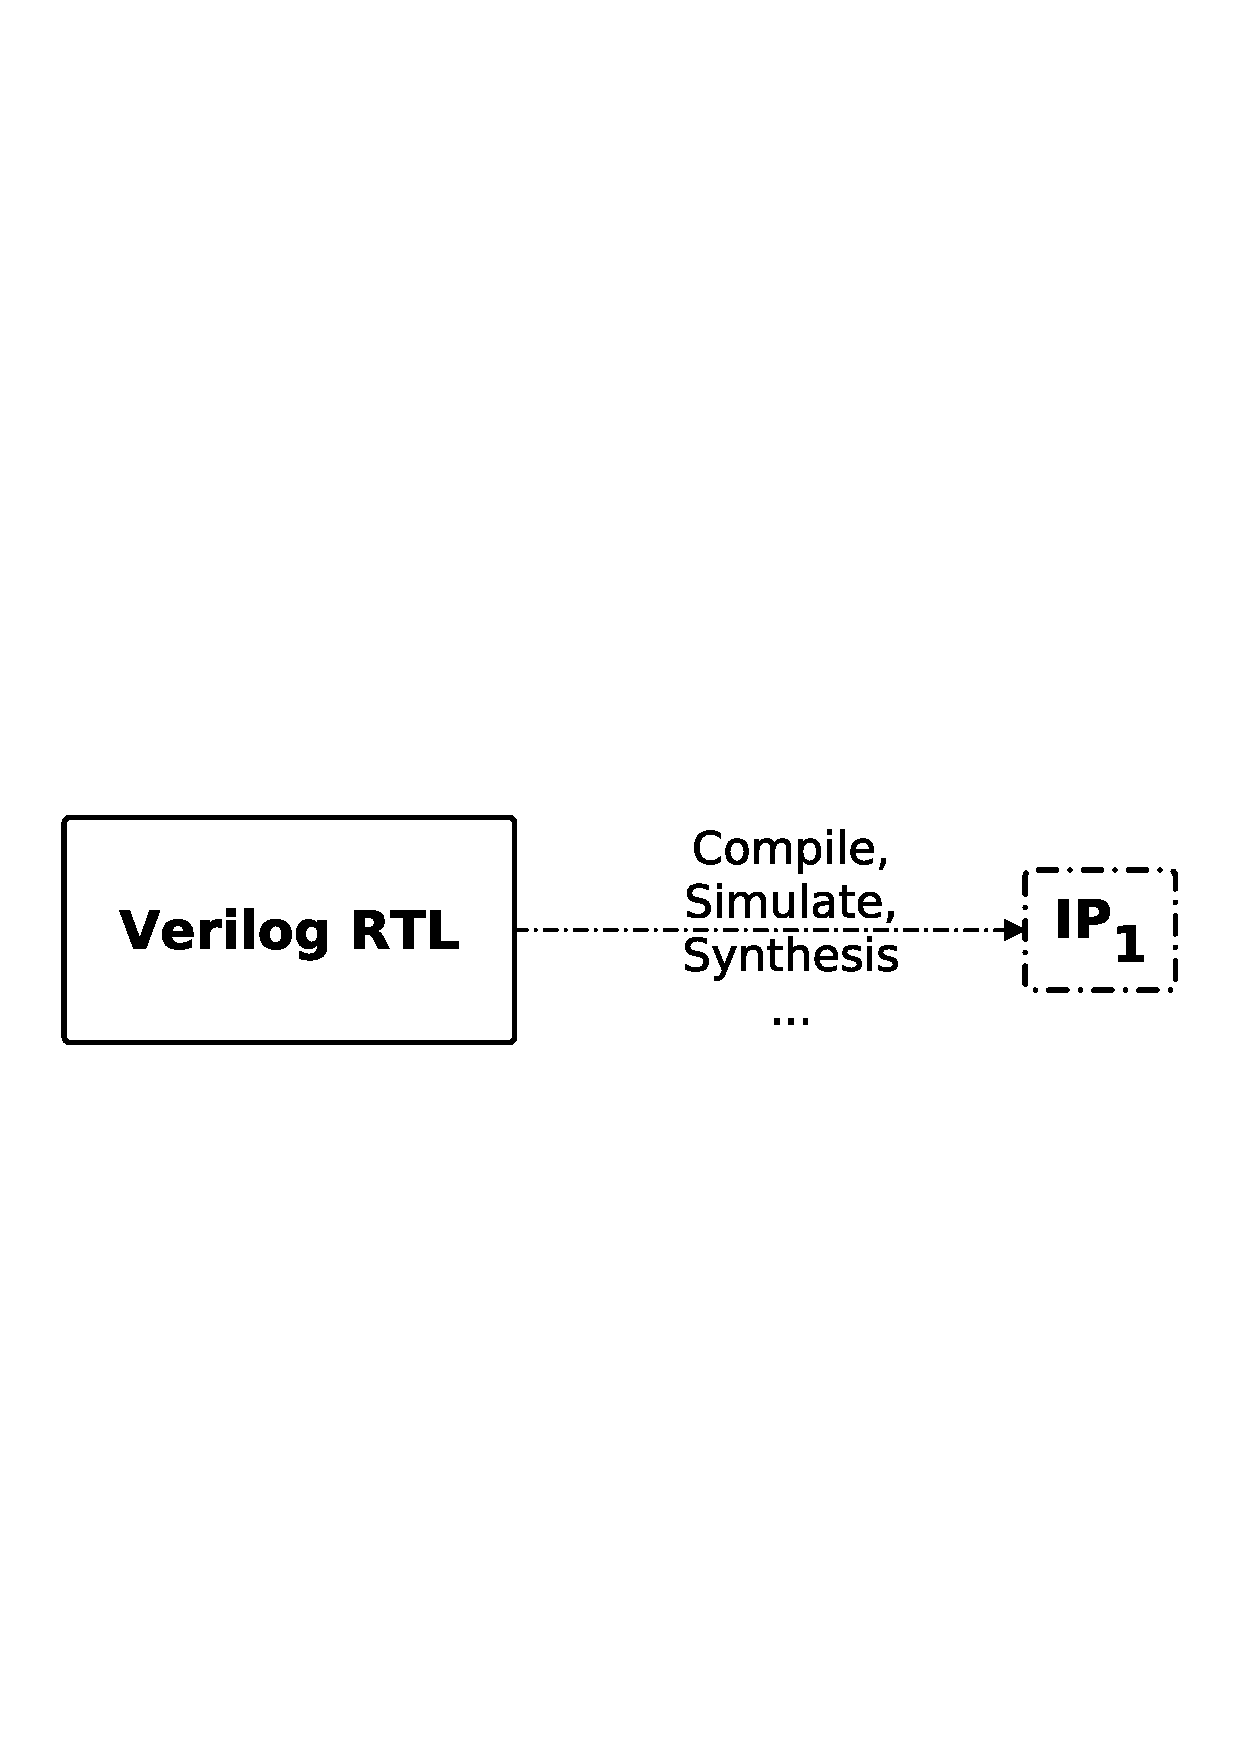
\includegraphics[width=0.5\columnwidth]{IPDesign}
%\vspace{-1ex}
\caption{Verilog Design Process}
%\vspace{-2ex}
\label{fig-ipdesign}
\end{figure}
\\
Things become different when use our precompiler. Fig\ref{fig-compiler}, as an example, shows the compiling process of the SV+ design.
\begin{figure}[h]
\centering
%\epsfig{file=}
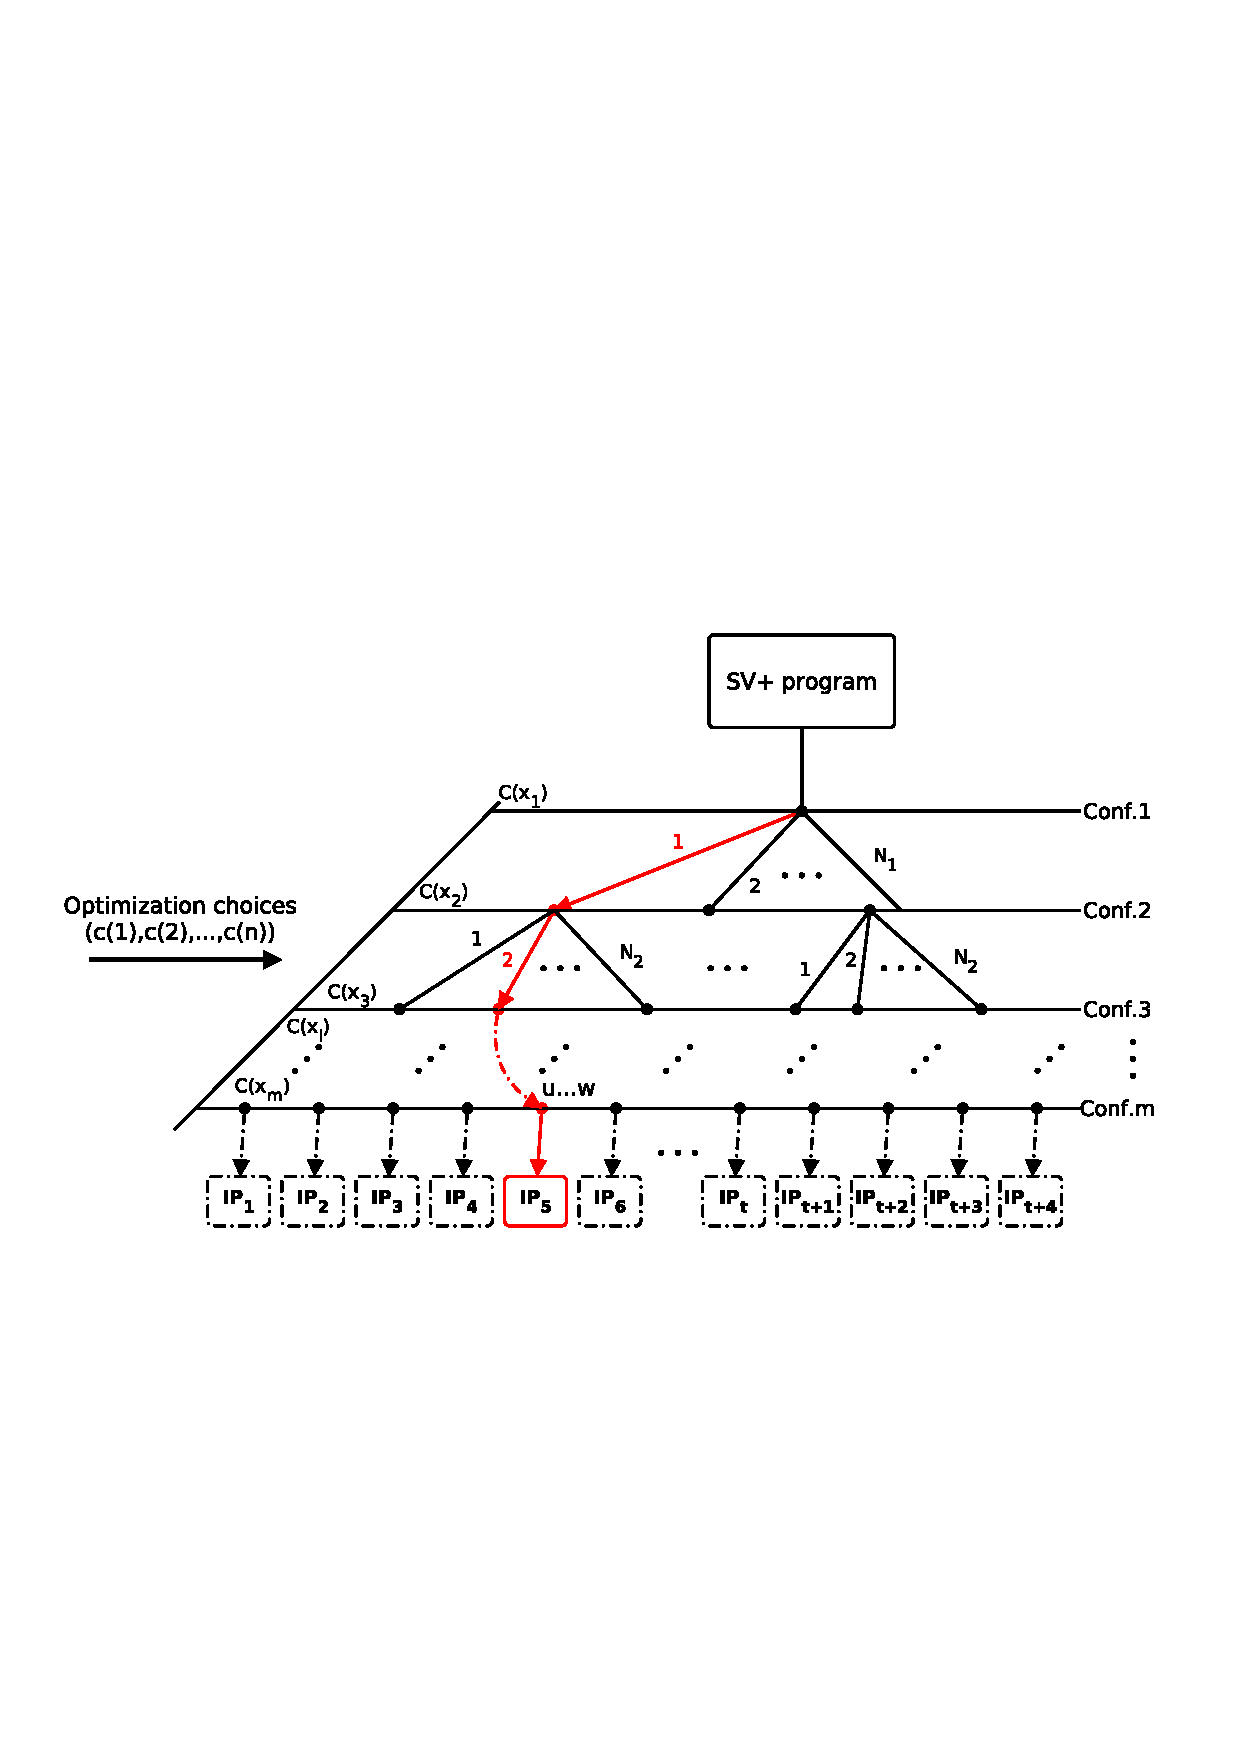
\includegraphics[scale=.4]{compileprocess}
\caption{SV+ Design process}
%\vspace{-2ex}
\label{fig-compiler}
\end{figure}
In this example, there are M reconfigurable structures in the SV+ description. The prcompiler scans the input program and parsers it firstly. M times of interactions lets the designer configure the circuit with M times' selections. And in each configuration stage, depends on the description, there are $N_i (1\leq i\leq M)$ options. So totally, we can have $\prod_{i=1}^{M}N_{i}$ kinds of configurations. They vary in resource cost and performance. Here in fig \ref{fig-compiler}, we suppose the designer inputs are $1,2,u...w$(the red line highlights the selections). Finally, he/she gets $\mathit{IP_5}$.
\\
Syntaxes and translations rules about how to construct the SV+ compiler can be found in appendix A.
